% This is samplepaper.tex, a sample chapter demonstrating the
% LLNCS macro package for Springer Computer Science proceedings;
% Version 2.20 of 2017/10/04
%
\documentclass[runningheads]{llncs}
%
\usepackage{graphicx}
\usepackage{todonotes}
\usepackage{verbatim}
\usepackage{caption}
% Used for displaying a sample figure. If possible, figure files should
% be included in EPS format.
%
% If you use the hyperref package, please uncomment the following line
% to display URLs in blue roman font according to Springer's eBook style:
% \renewcommand\UrlFont{\color{blue}\rmfamily}

\begin{document}
%
\title{Clustering Knowledge Graphs}
%
%\titlerunning{Abbreviated paper title}
% If the paper title is too long for the running head, you can set
% an abbreviated paper title here
%
\author{Lina Teresa Molinas Comet}
%
\authorrunning{Lina Teresa Molinas Comet.}
% First names are abbreviated in the running head.
% If there are more than two authors, 'et al.' is used.
%
\institute{RWTH Aachen University, Aachen, Germany \\
\email{lina.molinas.comet@rwth-aachen.de}\\
\url{http://dbis.rwth-aachen.de/cms}}
%
\maketitle              % typeset the header of the contribution
%
\begin{abstract}
The era of data is here and we need to deal with a big amount of data in different presentations or formats. It is necessary the extraction of data in order to get a specific information and with it give value to data and get the expected insights, making sense of data. There are some issues with big data, that need to be address, one way is graph representation of data. This task is not easy because of the amount of data, as well as the complexity on its representation. One way of representing information, and which is getting more common is graph-based because of its benefits (\todo{look for definition of graph and benefits, see if KG allows integration of information about entities from multiple sources, and if clustering of equivalent entities from diff sources is the key factor in the construction of KG }). But it is important to analyze and compare different clustering techniques and algorithms to get the most from this kind of representation. We will present the benefits of clustering on KG. We will present some common problems on graph clustering (like overlapping or inclusion of same entity in various clusters)
It is possible to use unsupervised techniques in order to explore large-datasets (\todo{rephrase it})
In this paper we present an overview of the most interesting techniques and algorithms design (approaches) with the purpose of improving clustering in graphs from a semantic perspective. We will revised in detail some of those algorithms in order to understand better, compare them and suggest the area of use specific to every case (presenting the pros and cons), and try to suggest the future of clustering.
Clustering is a valid tool to be use in the exploration of data (big amount of data, vast)

The abstract should briefly summarize the contents of the paper in
15--250 words.

\keywords{Knowledge Graphs \and Clustering \and Knowledge Bases \and Algorithms}
\end{abstract}
%
%
%
\section{Introduction}
Explain what and why is this paper here.

It is crucial to make sense of data but this task is challenged by the enormous amount of data in the era of information technology \cite{Pedrycz}

Various fields, such as intelligent data analysis (IDA), data mining, and system modeling attempt to assist the tasks involved in the understanding of data and discovery of tendencies on data \cite{Pedrycz}


\section{Background}
First of all, for a better understanding, it is important to clarify the main concepts related to the topic under study. In this section we present the core concepts associated with Knowledge Graphs and Clustering.
\subsection{Graphs}
\subsection{Knowledge Graphs}
Currently there is not a common definition of Knowledge Graphs and still exist some confusion on the use of the term, because of the Google's implementation of its own Knowledge Graph, which is a semantic complement to the search engine.\cite{Ehrlinger}. More over, \cite{Ehrlinger} emphasizes that the definitions in the context of Knowledge Graphs by the Journal of Web Semantics and by the Semantic Web Company could be used to refer to the definition of Ontology without involving graph structures. 
In the definition presented by \cite{Paulheim}, "a knowledge graph
1) mainly describes real world entities and their interrelations, organized in a graph, 2) defines possible classes and relations of entities in a schema, 3) allows for potentially interrelating arbitrary entities with each other, and 4) covers various topical domains". A more formal definition which is also more focused on the context of Linked Data, is the one proposed by \cite{Farber} "Since in the Semantic Web RDF graphs are used we use the term knowledge graph for any RDF graph. An RDF graph consists of a finite set of RDF triples where each RDF triple (s, p, o) is an ordered set of the following RDF terms: a subject s ∈ U ∪ B, a predicate p ∈ U, and an object o ∈ U ∪ B ∪ L. An RDF term is either a URI u ∈ U, a blank node b ∈ B,or a literal l ∈ L. U, B, and L are infinite sets and pairwise disjoint".
It is important to observe, the confusions related to the use of the term, as described in \cite{Ehrlinger}, when using interchangeably the terms Knowledge Bases, Knowledge Vault, Knowledge Graphs, and Ontology, as well as when referring to the implementation of Google’s Knowledge Graph. While there exists differences between the scope and techniques used in each of those terms.
\subsection{Knowledge-based systems}
A knowledge-based system is also called an expert system, and is part of one of the areas of Artificial Intelligence.\cite{Tripathi}
On the other hand, \cite{Engelmore} indicates that a knowledge base it can be described as a global data base which is part of the implementation dimension of an expert system, and that contains among others: facts, rules, and relations. Moreover, \cite{Engelmore} mentions that one of the key profit of having an expert system is the improvement on quality of the tasks related to decision making.
The expert systems aim to acquire expert knowledge in the context of a particular domain. That knowledge comes from a human expert and then is available to other users which does not have such expertise. \cite{Tripathi}

\subsection{Clustering}
Clustering has become a valid and well-establish tool to make sense of the big amount of data that we face nowadays, and helps to take decision based on data. Clustering helps in the exploration of huge amount of data. \cite{Pedrycz}

The use of clustering is well-suite for a variety of areas of application, for instance: engineering, economics, finance, biomedicine, biological sciences, etc. \cite{Pedrycz}

The optimization in clustering is predominantly data-oriented. \cite{Pedrycz}
It is required to be careful in the selection of algorithms and concepts 

\subsection{Distance and Similarity}

\subsection{Other concepts}

\section{State of the Art}
In this section we present novel and also more traditional techniques and algorithms used in the field of Knowledge Graph clustering. 

\subsection{General Techniques for Knowledge Graph Clustering}
Presentation of well-known techniques for graph clustering.

\subsection{Techniques and Algorithms}
Revision in more detail the selected algorithms and techniques 
\subsubsection{Graph clustering for content aggregation for an Ontology-Based P2PKM}
Present the work of \cite{Schmitz} where they introduce the approach of semantic self-descriptions to be publish among peers and for which they use a clustering algorithm to obtain that self-description.

\subsubsection{Structural similarity clustering entities}

\subsubsection{Entity Clustering using link features}

\begin{center}
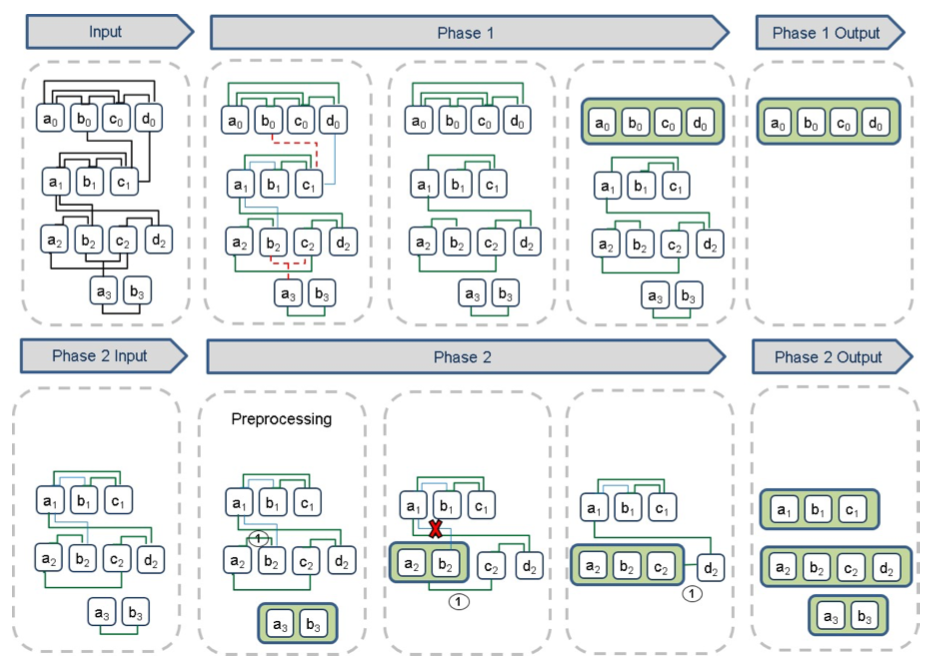
\includegraphics[width=1\textwidth]{clip_example.png}
\captionof{figure}{Example of CLIP \cite{Saeedi}}
\end{center}

\begin{center}
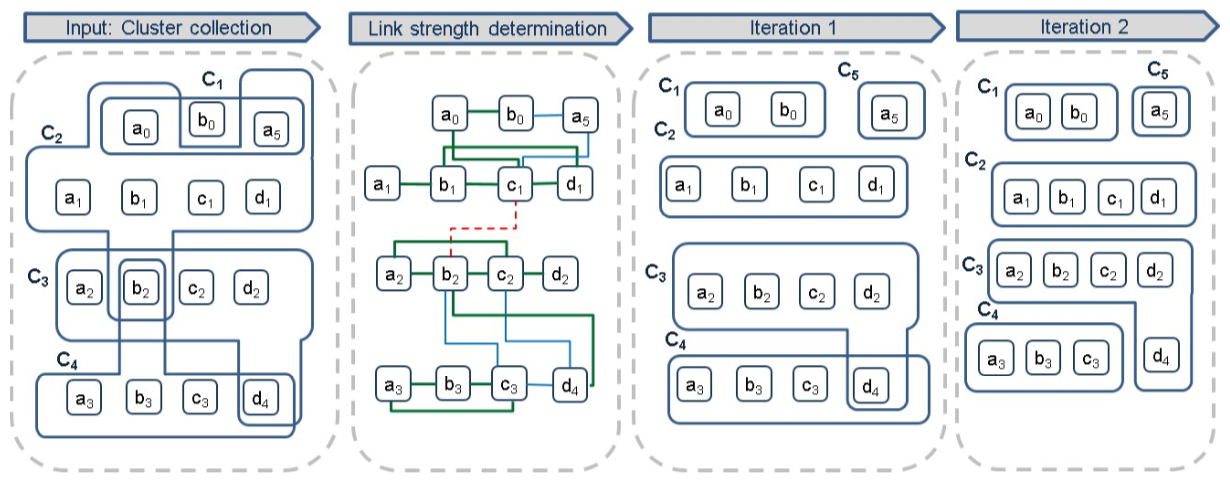
\includegraphics[width=1\textwidth]{clip_overlap_resolution.png}
\captionof{figure}{Overlapping resolution on CLIP \cite{Saeedi}}
\end{center}




\section{Analysis and comparison of presented approaches}
\section{Discussion}
\section{Conclusion}

%
% ---- Bibliography ----
%
% BibTeX users should specify bibliography style 'splncs04'.
% References will then be sorted and formatted in the correct style.
%
% \bibliographystyle{splncs04}
% \bibliography{mybibliography}
%
\begin{thebibliography}{8}
\bibitem{Schmitz}
Schmitz, C., Hotho, A., J{\"a}schke, R., Stumme, G.: Content Aggregation on Knowledge Bases Using Graph Clustering. In: Sure, Y., Domingue, J. (eds.) The Semantic Web: Research and Applications. ESWC 2006, LNCS, vol. 4011, pp. 530--544.
Springer, Berlin, Heidelberg (2006). \doi{10.1007/11762256\_39}

\bibitem{Elbattah}
Elbattah, M., Roushdy, M., Aref, M., M.Salem, A.: Large-Scale Entity Clustering Based on Structural Similarity within Knowledge Graphs. In: Arun, K., Somani, G. (eds.) Big Data Analytics: Tools and Technology for Effective Planning, Edition: 1, Chapter: 14, pp. 311--334. CRC Press Editors (2017). \doi{10.1201/b21822-14}

\bibitem{Saeedi}
Saaedi, A., Peukert, E., Rahm, E.  : Using Link Features for Entity Clustering in Knowledge Graphs. In: Gangemi, A., Navigli, R., Vidal, M., Hitzler, P., Troncy, R., Hollink, L., Tordai, A., Alam, M. (eds.) The Semantic Web. ESWC 2018, LNCS, vol. 10843, pp. 576--592.
Springer International Publishing, Cham (2018). \doi{10.1007/978-3-319-93417-4\_37}

\bibitem{Pedrycz}
Pedrycz, W.: Knowledge-Based Clustering: From Data to Information Granules. 2nd edn. Wiley-Interscience, New York, NY, USA (2005)

\bibitem{Zhang}
Zhang, X., Lv, Y., Lin, E : Object Clustering in Linked Data using Centrality. In: Proceedings of China Conference on Knowledge Graph and Semantic Computing (CCKS2016)
on Proceedings, pp. 172--183. Publisher, Location (2016). \doi{10.1007/978-981-10-3168-7\_17}

\bibitem{Ehrlinger}
Ehrlinger, L, W{\"o}{\ss}, W.: Towards a Definition of Knowledge Graphs. In: Martin, M., Cuquet M., Folmer, E. (eds.) In Joint Proceedings of the Posters and Demos Track of the 12th International Conference on Semantic Systems - SEMANTiCS2016 and the 1st International Workshop on Semantic Change \& Evolving Semantics (SuCCESS'16), CEUR-WS, vol. 1695, Leipzig, Germany (2016). \doi{10.10007/1234567890}

\bibitem{Paulheim}
Paulheim, H.: Knowledge Graph Refinement: A Survey of Approaches and Evaluation Methods. Semantic Web Journal, 489--508 (2017). \doi{10.3233/SW-160218}

\bibitem{Farber}
F{\"a}rber, M., Bartscherer, F, Menne,C., Rettinger, A.: Linked data quality of DBpedia, Freebase, OpenCyc, Wikidata, and YAGO. Semantic Web Journal, 77--129 (2018). \doi{10.3233/SW-170275}

\bibitem{Tripathi}
Tripathi, K.: A Review on Knowledge-based Expert System: Concept and Architecture. IJCA Special Issue on Artificial Intelligence Techniques-Novel Approaches \& Practical Applications (2011). \doi{10.5120/2845-226}

\bibitem{Engelmore}
Engelmore R.S.  : Artificial Intelligence and Knowledge Based Systems: Origins, Methods and Opportunities for NDE. In: Thompson D.O., Chimenti D.E. (eds.) Review of Progress in Quantitative Nondestructive Evaluation. Review of Progress in Quantitative Nondestructive Evaluation, vol. 6 A., 
Springer, Boston, MA (1987). \doi{10.1007/978-1-4613-1893-4\_1}


\end{thebibliography}

\begin{comment}
\bibitem{ref_lncs1}
Author, F., Author, S.: Title of a proceedings paper. In: Editor,
F., Editor, S. (eds.) CONFERENCE 2016, LNCS, vol. 9999, pp. 1--13.
Springer, Heidelberg (2016). \doi{10.10007/1234567890}

\bibitem{ref_article1}
Author, F.: Article title. Journal \textbf{2}(5), 99--110 (2016)

\bibitem{ref_book1}
Author, F., Author, S., Author, T.: Book title. 2nd edn. Publisher,
Location (1999)

\bibitem{ref_proc1}
Author, A.-B.: Contribution title. In: 9th International Proceedings
on Proceedings, pp. 1--2. Publisher, Location (2010)

\bibitem{ref_url1}
LNCS Homepage, \url{http://www.springer.com/lncs}. Last accessed 4
Oct 2017

\end{comment}
\end{document}


